% !TEX program = xelatex
\documentclass[12pt]{report}
\usepackage{fontspec}

\defaultfontfeatures{Ligatures=TeX}
% \setmainfont{DidactGothic-Regular}
\setmainfont{NotoSans-Regular}


\usepackage[english, bulgarian]{babel}
\usepackage{indentfirst}
\usepackage[a4paper, portrait, margin = 2.0 cm]{geometry}
\usepackage{url}
\usepackage{color}
\usepackage{float}
\usepackage{xcolor}
\usepackage{graphicx}
\usepackage{listings}
\usepackage{subfig}
\usepackage[export]{adjustbox}

\def\changemargin#1#2{\list{}{\rightmargin#2\leftmargin#1}\item[]}
\let\endchangemargin=\endlist 

\renewcommand{\baselinestretch}{1.1}
\setlength{\emergencystretch}{3em}

\usepackage{graphicx}
\graphicspath{ {./resources/} }

\lstset{
	backgroundcolor = \color{light-gray},
    language = C,
    xleftmargin = 1cm,
    framexleftmargin = 1em,
    basicstyle=\ttfamily,
	moredelim=[is][\underbar]{_}{_},
}

\usepackage{color}
\definecolor{Bluish}{rgb}{0.39,0.55,0.78}
\definecolor{light-gray}{gray}{0.9}

\usepackage{hyperref}
\hypersetup{
    colorlinks=true,
    linktoc=all,
    citecolor=black,
    filecolor=black,
    linkcolor=black,
    urlcolor=black
}

\usepackage{tabularx}


\title{Дипломна работа}
\author{Диана Генева <dageneva@qtrp.org>}
\date{2018}

\begin{document}
\maketitle
\thispagestyle{empty}
\tableofcontents
\pagebreak

\chapter{Нулева зона}
Бла, бла, бла, аз съм толкова емоционална. 
Не знам

\includegraphics[width=0.5\textwidth ]{pikachu}

\chapter{Емоции в реч}
    \section{Физика на тъгата}
    $https://www.clear.rice.edu/elec301/Projects01/speech_syn/sourcefilter.htm$

    Едно-две изречения на защо искаме да опишем конфигурацията на вокалния тракт.
    и какво е вокалния тракт.

    \begin{figure}[ht]%
        \centering
        \begin{changemargin}{0cm}{0cm} 
            \subfloat[Part 1]{%
                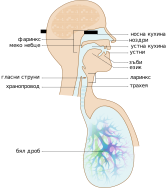
\includegraphics[width=0.48\paperwidth,valign=t]{physics}%
            } \hspace{0.8cm}
            \subfloat[Part 2]{%
                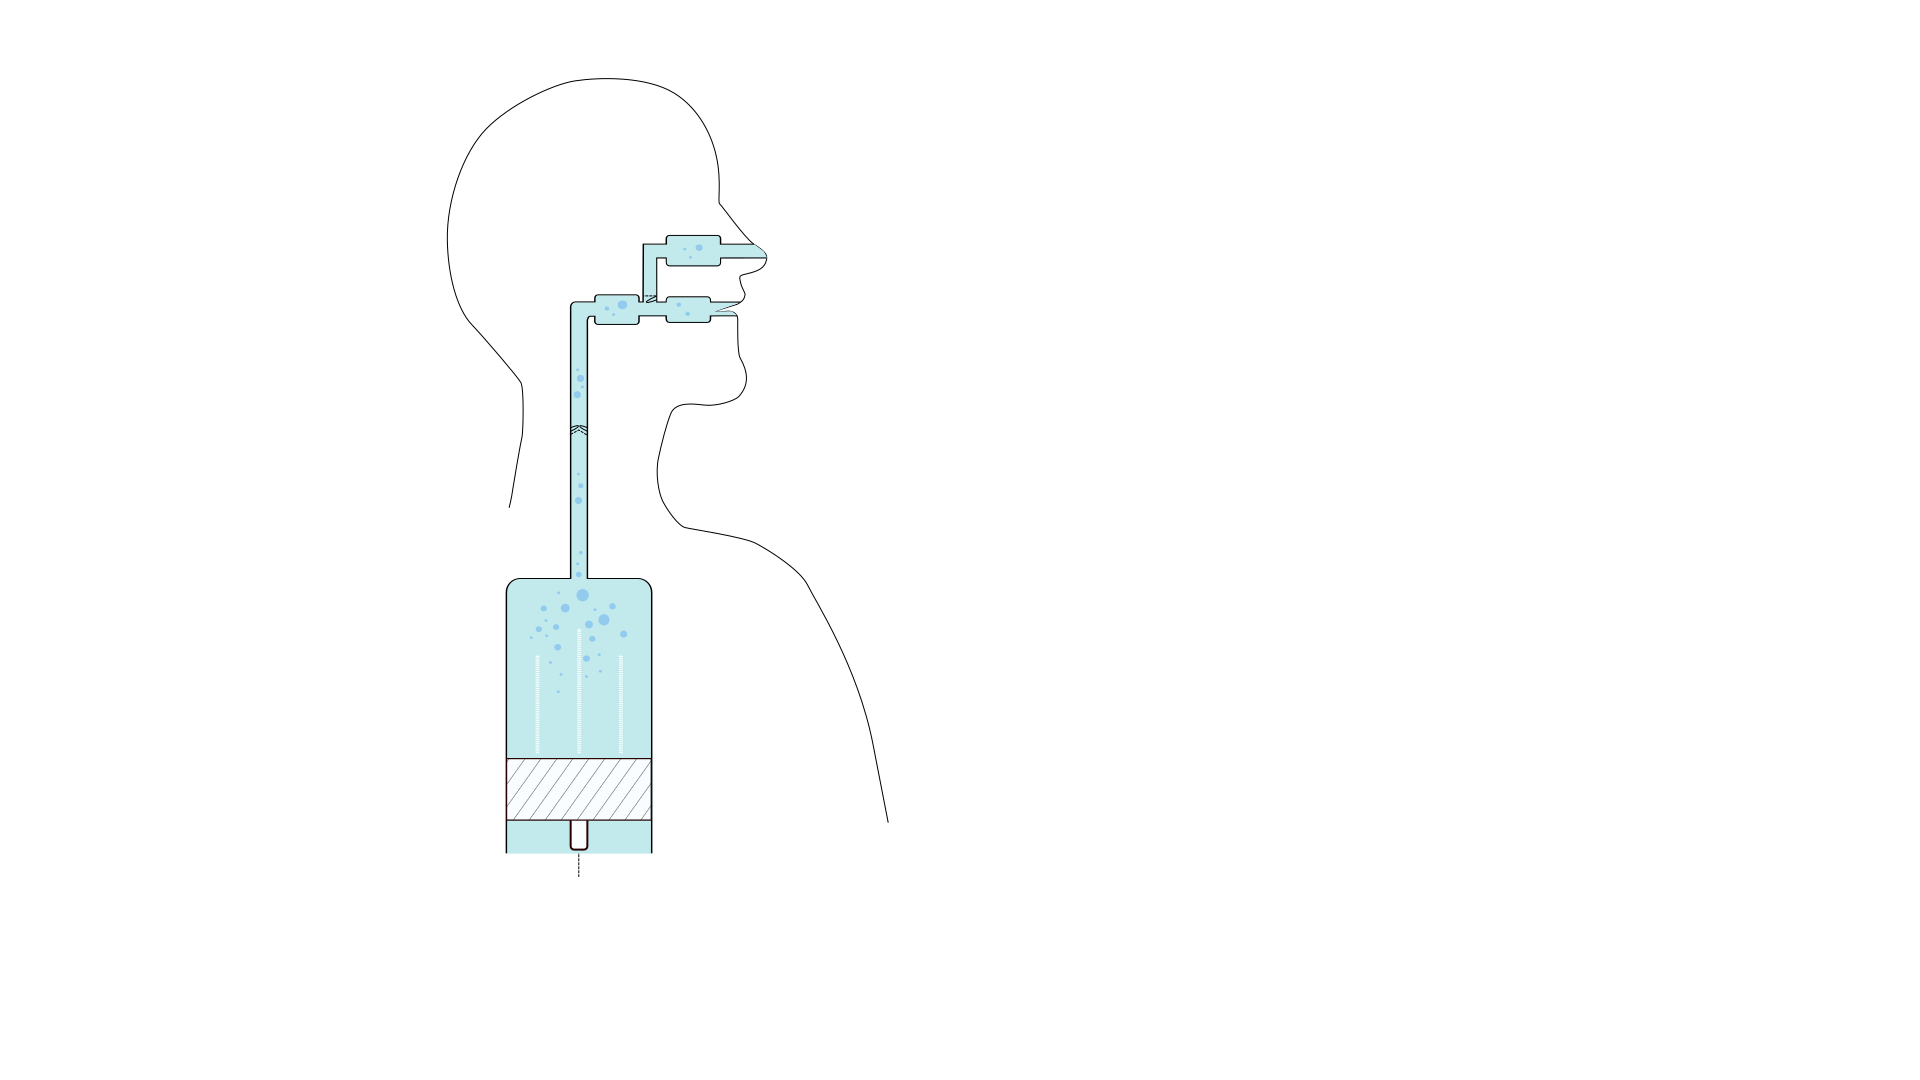
\includegraphics[width=0.28\paperwidth,valign=t]{tubes}%
                \vphantom{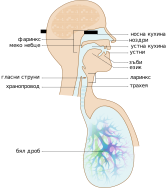
\includegraphics[width=0.48\paperwidth,valign=t]{physics}}%
            }
        \end{changemargin} 

        \caption{Гррррр}%
        \label{fig:example}%
    \end{figure}
    
    Да разгледаме Фиг.1 като цялостна система за производство на реч.
    Речта, всъщност, представлява просто акустичната вълна, получена на края на системата - устни и ноздри - в следствие на изкарания от белия дроб въздух.

    Белият дроб работи като енергиен източник за тази системата - въздушният поток, получен при свиването му от междуребрените мускули и диафрагмата,
    се пропагира нагоре по трахеята и през глотиса (отворе между гласните струни). Тъй като налягането в глотиса е по-малко от това в който и да е от двата му края, по закона на Бернули
    в някакъв момент става толкова ниско, че позволява на гласните струни да се затворят. В следствие се натрупва налягане зад гласните струни, което в някакъв момент ги принуждава
    да се отворят и цикълът се повтаря отначало. В резултат се получава осцилиране на гласните струни. Честотата на отварянето и затварянето зависи от анатомични особености като еластичността и големината на
    гласните струни, налягането в белия дроб и други. При мъжете тази честота е средно 125 Hz, а при жените - 210 Hz. Акустичната вълна, която се получава в следствие на осцилацията,
    преминава през вокалния тракт, където се завихря, при срещане на прегради, като устни и зъби, и в крайна сметка напуска системата през някой от отворите.

    При целият този процес се губи част от енергията, поради различни фактори: стените на вокалния тракт са меки и еластични, радиацията на вълната при устните и ноздрите и други.

    В зависимост от начинът, по който вълната напуска системата, можем да класифицираме произведените звуци по следния начин:

    \section{Загладено опростяване}    
    \section{Характеристики}
        \subsection{Избор}
        \subsection{Извличане}
    \section{Класификация}    
    \section{Резултати}

\chapter{Грубо в мозъка}
    \section{Характеристики}
        \subsection{Избор}
        \subsection{Извличане}
    \section{Класификация}    
    \section{Резултати}
\chapter{Двойната звезда}
    \section{Резултати}
\chapter{Големият портрет}


\end{document}